% ------------------------------------------------------------------------------
% TYPO3 Version 10.0 - What's New (English Version)
%
% @author	Michael Schams <schams.net>
% @license	Creative Commons BY-NC-SA 3.0
% @link		http://typo3.org/download/release-notes/whats-new/
% @language	English
% ------------------------------------------------------------------------------

\section{Changes for Integrators}
\begin{frame}[fragile]
	\frametitle{Changes for Integrators}

	\begin{center}\huge{Chapter 3:}\end{center}
	\begin{center}\huge{\color{typo3darkgrey}\textbf{Changes for Integrators}}\end{center}

\end{frame}

% ------------------------------------------------------------------------------
% TYPO3 Version 10.0 - Breaking Changes

\begin{frame}[fragile]
	\frametitle{Changes for Integrators}
	\framesubtitle{Breaking Changes}

	\small
		Integrators be advised: In TYPO3 v9, some PHP code, TSconfig, TypoScript
		options and conditions, as well as scheduler tasks were marked deprecated.

		\vspace{0.2cm}

		In accordance to TYPO3's \textbf{deprecation policy}, these components have
		changed or have been removed in TYPO3 v10.0.

		\vspace{0.2cm}

		Enable the deprecation log, carefully test your code and review the log to
		locate possible issues. Use the built-in
		\href{https://docs.typo3.org/m/typo3/reference-coreapi/master/en-us/ApiOverview/ExtensionScanner/Index.html}{Extension Scanner}
		to get a full report of extension incompatibilities.

	\normalsize

\end{frame}

% ------------------------------------------------------------------------------
% Feature | 78432 | Add log message for Switch User action

\begin{frame}[fragile]
	\frametitle{Changes for Integrators}
	\framesubtitle{Backend User Switch}

	\begin{itemize}
		\item A log message is written if an admin user switches to another backend user:
	\end{itemize}

	\begin{figure}
		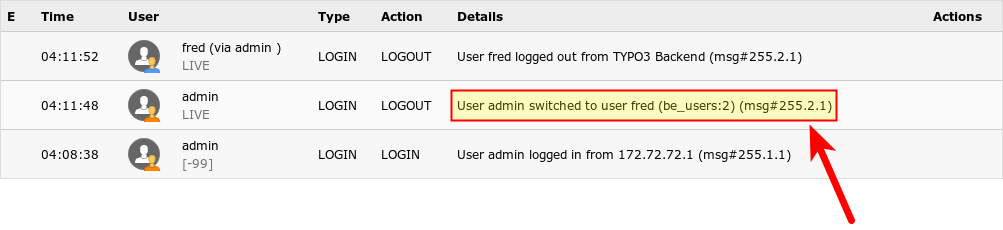
\includegraphics[width=0.90\linewidth]{ChangesForIntegrators/78432-SwitchUserActionLogMessage.png}
	\end{figure}

\end{frame}

% ------------------------------------------------------------------------------
% Feature | 83734 | Add support for current page in configcache
% Breaking | 88564 | PageTSconfig setting TSFE.constants removed
% Breaking | 88657 | Popup configuration in FormEngine dropped

\begin{frame}[fragile]
	\frametitle{Changes for Integrators}
	\framesubtitle{TypoScript Changes}

	\begin{itemize}
		\item TypoScript property \texttt{config.cache} now supports keyword
			"\texttt{current}" to refer to the current page. For example:\newline
			\smaller\texttt{config.cache.all = fe\_users:current}\normalsize

		\item The Page/User TSconfig setting \texttt{TSFE.constants} has been removed.

			\begin{itemize}\smaller
				\item[\ding{228}] Include TypoScript conditions in setup/constants and use a proper configuration in file \texttt{ext\_localconf.php}.
			\end{itemize}

		\item The following two options to configure the size of popup windows have been removed:

			\begin{itemize}
				\item \texttt{options.popupWindowSize}
				\item \texttt{options.rte.popupWindowSize}
			\end{itemize}

	\end{itemize}

\end{frame}

% ------------------------------------------------------------------------------
% Breaking | 88640 | Database field sys_template.nextLevel and TypoScript sublevel inheritance removed
% Task | 88755 | Remove POST option from typolink.addQueryString

\begin{frame}[fragile]
	\frametitle{Changes for Integrators}
	\framesubtitle{TypoScript Changes}

	\begin{itemize}
		\item The database field \texttt{nextLevel} of the database table
			\texttt{sys\_template} has been removed.

			\begin{itemize}\smaller
				\item[\ding{228}] Replace the record (the UID is stored in the field \texttt{nextLevel}) with a condition to add TypoScript for subpages. For example: \texttt{[tree.level > 1]}
			\end{itemize}\normalsize

		\item The following values are \textbf{not allowed} anymore:

			\begin{itemize}\smaller
				\item \texttt{typolink.addQueryString.method = POST}
				\item \texttt{typolink.addQueryString.method = GET,POST}
				\item \texttt{typolink.addQueryString.method = POST,GET}
			\end{itemize}\normalsize

			\begin{itemize}\smaller
				\item[\ding{228}] Change the assignments in TypoScript, Fluid and PHP to \texttt{GET}.
			\end{itemize}\normalsize

	\end{itemize}

\end{frame}

% ------------------------------------------------------------------------------
% Breaking | 87583 | Remove obsolete APC Cache Backend implementation
% Breaking | 87558 | Consolidate extbase caches

\begin{frame}[fragile]
	\frametitle{Changes for Integrators}
	\framesubtitle{Caches}

	% decrease font size for code listing
	\lstset{basicstyle=\tiny\ttfamily}

	\begin{itemize}
		\item Caching framework does not support the \texttt{ApcBackend} anymore

			\begin{itemize}\smaller
				\item[\ding{228}] Use \textbf{APCu} instead - note the "u".
			\end{itemize}

\begin{lstlisting}
OLD:
$GLOBALS['TYPO3_CONF_VARS']['SYS']['caching']['cacheConfigurations']['rootline']['backend'] =
\TYPO3\CMS\Core\Cache\Backend\ApcBackend::class;

NOW:
$GLOBALS['TYPO3_CONF_VARS']['SYS']['caching']['cacheConfigurations']['rootline']['backend'] =
\TYPO3\CMS\Core\Cache\Backend\ApcuBackend::class;
\end{lstlisting}

		\item Extbase caches \texttt{extbase\_reflection} and \texttt{extbase\_datamapfactory\_datamap}
			have been consolidated and are now available as a single cache named "\texttt{extbase}".

	\end{itemize}

\end{frame}

% ------------------------------------------------------------------------------
% Breaking | 87009 | Use multiple translation files by default in EXT:form

\begin{frame}[fragile]
	\frametitle{Changes for Integrators}
	\framesubtitle{Form Framework}

	% decrease font size for code listing
	\lstset{basicstyle=\tiny\ttfamily}

	\begin{itemize}
		\item The following option has been renamed:\newline
			\small\texttt{translationFile} \textrightarrow\hspace{0.1cm}\texttt{translationFiles}\normalsize
		\item The default translation files are now registered at index 10:

			\begin{itemize}
				\item \texttt{EXT:form/Resources/Private/Language/locallang.xlf}
				\item \texttt{EXT:form/Resources/Private/Language/Database.xlf}
			\end{itemize}

		\item Custom form YAML configuration files need to be updated.

\begin{lstlisting}
OLD:
translationFile: path/to/locallang.xlf

NEW:
translationFiles:
  20: path/to/locallang.xlf
\end{lstlisting}

	\end{itemize}

\end{frame}

% ------------------------------------------------------------------------------
% xxxxx | Cache Storage Type

\begin{frame}[fragile]
	\frametitle{Changes for Integrators}
	\framesubtitle{Cache Storage Type (1)}

	\begin{itemize}

		\item TYPO3 features a flexible caching system with a default configuration
			that is ideal for most use cases.
		\item The storage type can now be configured to fine-tune the caches and
			increase performance depending on the individual environment.

			\begin{itemize}
				\item Choose the \textbf{database} storage for a standard environment
					or if a network file system (NFS) is used for example.
				\item Choose the \textbf{file system} if a distributed database setup
					is used for example.
				\item Choose \textbf{custom cache settings} to configure the storage
					type for each cache independently.
			\end{itemize}

		\item For more complex installations, memory-based caches such as
			\href{https://redis.io/}{Redis}
			or
			\href{https://memcached.org/}{Memcached}
			should be considered.

	\end{itemize}

\end{frame}

% ------------------------------------------------------------------------------
% xxxxx | Cache Storage Type

\begin{frame}[fragile]
	\frametitle{Changes for Integrators}
	\framesubtitle{Cache Storage Type (2)}

	\begin{itemize}

		\item Backend: \textbf{MAINTENANCE} \ding{223}\hspace{0.1cm}\textbf{Settings} \ding{223}\hspace{0.1cm}\textbf{Cache}:
		\end{itemize}

	\begin{figure}
		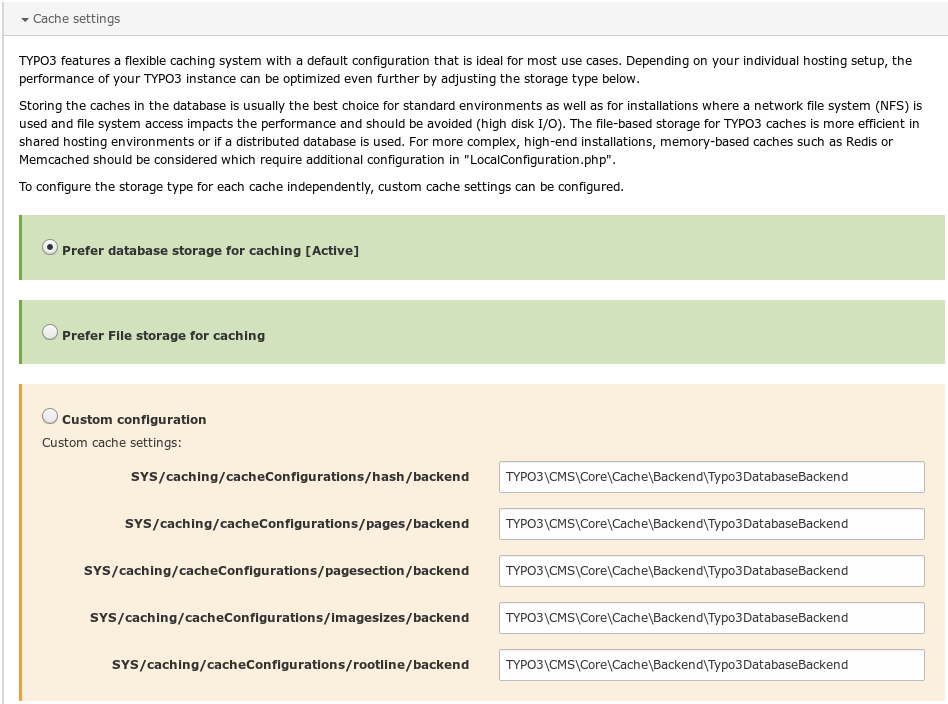
\includegraphics[width=0.60\linewidth]{ChangesForIntegrators/xxxxx-CacheStorageType.png}
	\end{figure}

\end{frame}

% ------------------------------------------------------------------------------
% 87499 | Drop extensions "taskcenter" and "sys_action" from core

\begin{frame}[fragile]
	\frametitle{Changes for Integrators}
	\framesubtitle{Task Center and \texttt{EXT:sys\_action}}

	\begin{itemize}

		\item The system extensions \texttt{EXT:taskcenter} and \texttt{EXT:sys\_action}
			have been removed from the core.

		\item They are now available as separate extensions from the
			\href{https://extensions.typo3.org/}{TER}
			and at
			\href{https://github.com/FriendsOfTYPO3}{GitHub}.

		\item Keep an eye on the
			\href{https://typo3.org/community/teams/typo3-development/initiatives/typo3-dashboard-initiative/}{Dashboard Initiative}
			for a new and much better approach.

	\end{itemize}

\end{frame}

% ------------------------------------------------------------------------------
% Feature | 88648 | Define Twitter Card Type In Page Properties
% Important | 86577 | Query parameters are now included in canonicalized URLs

\begin{frame}[fragile]
	\frametitle{Changes for Integrators}
	\framesubtitle{Miscellaneous (1)}

	% decrease font size for code listing
	\lstset{basicstyle=\tiny\ttfamily}

	\begin{itemize}

		\item Type of Twitter Card can be selected/configured now.
			This option renders the meta tag \texttt{twitter:card} in the frontend.

\begin{lstlisting}
page {
  meta {
    twitter:card = summary_large_image
    twitter:card.replace = 1
  }
}
\end{lstlisting}

		\item Only parameters that are needed to calculate the cHash are included in canonicalized URLs by default.
			Additional query parameters can now be configured:

\begin{lstlisting}
$GLOBALS['TYPO3_CONF_VARS']['FE']['additionalCanonicalizedUrlParameters'].
\end{lstlisting}

		\smaller
			Note: only add parameters which change the content of your page. Otherwise search engines will likely classify your pages as duplicate content.
		\normalsize

	\end{itemize}

\end{frame}

% ------------------------------------------------------------------------------
% Breaking | 88681 | Import Of PHP Files In Import Export Files Removed
% Breaking | 88500 | RTE image handling functionality dropped
% Breaking | 81950 | Remove leftover workspaces unpublishing functionality

\begin{frame}[fragile]
	\frametitle{Changes for Integrators}
	\framesubtitle{Miscellaneous (2)}

	% decrease font size for code listing
	\lstset{basicstyle=\tiny\ttfamily}

	\begin{itemize}

		\item When importing XML data using \texttt{EXT:impexp}, the File Deny Pattern applies
			now and rejects embedded PHP files for example.

		\item RTE image handling functionality has been removed completely.
			For image support in CKEditor, consider to use \texttt{EXT:rte\_ckeditor\_image} for example.

		\item A property within workspaces for \textit{unpublishing} records has been removed in v10
			(including the database field \texttt{sys\_workspace.unpublish\_time}). This feature was
			disabled in TYPO3 v4.5 and not used or provided by the TYPO3 core.

	\end{itemize}

\end{frame}

% ------------------------------------------------------------------------------
% Breaking | 88772 | JavaScript script tags omit type=text/javascript in HTML5
% Remove system extension EXT:rsaauth
% Remove system extension EXT:fe_edit

\begin{frame}[fragile]
	\frametitle{Changes for Integrators}
	\framesubtitle{Miscellaneous (3)}

	% decrease font size for code listing
	\lstset{basicstyle=\tiny\ttfamily}

	\begin{itemize}

		\item When rendering HTML5 output, \texttt{<script>} tags do not include
			the attribute \texttt{type="text/javascript"} anymore.

		\item This can be re-enabled for the frontend by using TypoScript if required:

\begin{lstlisting}
page {
  includeJS {
    myfile = EXT:example/Resources/Public/JavaScript/myfile.js
    myfile.type = text/javascript
  }
}
\end{lstlisting}

		\item The following deprecated system extensions have been removed:

			\begin{itemize}
				\item \texttt{EXT:rsaauth}
				\item \texttt{EXT:fe\_edit}
			\end{itemize}

	\end{itemize}

\end{frame}

% ------------------------------------------------------------------------------
